\documentclass[11pt]{article}
\usepackage{latexsym}
\usepackage{amsmath}
\usepackage{amssymb}
\usepackage{amsthm}
\usepackage{epsfig}
\usepackage{bm}
\usepackage{scrextend}
\usepackage[tight]{subfigure}
\usepackage{physics}

\usepackage{amsmath}
% \usepackage{algorithmic}
% \usepackage{algorithm}
% \usepackage{algpseudocode}
\usepackage{algorithm}
 %on linux you may need to run sudo apt-get install texlive-full to install algorithm.sys
\usepackage{algorithmic}

\DeclareMathOperator*{\minimize}{min}
\DeclareMathOperator*{\maximize}{max}


\usepackage{verbatim}

\newcommand{\handout}[5]{
  \noindent
  \begin{center}
  \framebox{
    \vbox{
      \hbox to 5.78in { {#1} \hfill #2 }
      \vspace{4mm}
      \hbox to 5.78in { {\Large \hfill #5  \hfill} }
      \vspace{2mm}
      \hbox to 5.78in { {\em #3 \hfill #4} }
    }
  }
  \end{center}
  \vspace*{4mm}
}

\newcommand{\lecture}[5]{\handout{#1}{#2}{#3}{#4}{#5}}
\newcommand{\collision}[0]{\mathrm{collision}}
\newcommand{\nocollision}[0]{\overline{\collision}}
\newcommand{\argmin}[1]{\underset{#1}{\operatorname{arg}\,\operatorname{min}}\;}
\newcommand{\argmax}[1]{\underset{#1}{\operatorname{arg}\,\operatorname{max}}\;}
\newcommand*{\QED}{\hfill\ensuremath{\square}}

\newtheorem{theorem}{Theorem}
\newtheorem{corollary}[theorem]{Corollary}
\newtheorem{lemma}[theorem]{Lemma}
\newtheorem{observation}[theorem]{Observation}
\newtheorem{proposition}[theorem]{Proposition}
\newtheorem{definition}[theorem]{Definition}
\newtheorem{claim}[theorem]{Claim}
\newtheorem{fact}[theorem]{Fact}
\newtheorem{assumption}[theorem]{Assumption}
\newtheorem{note}[theorem]{Note}

% 1-inch margins, from fullpage.sty by H.Partl, Version 2, Dec. 15, 1988.
\topmargin 0pt
\advance \topmargin by -\headheight
\advance \topmargin by -\headsep
\textheight 8.9in
\oddsidemargin 0pt
\evensidemargin \oddsidemargin
\marginparwidth 0.5in
\textwidth 6.5in

\parindent 0in
\parskip 1.5ex
%\renewcommand{\baselinestretch}{1.25}

\begin{document}

\lecture{Statistical Techniques in Robotics (16-831, S22)}{Lecture \#08
  (Monday, February 14)}{Lecturer: Kris Kitani}{Scribes: Feng Xiang, Yuqing Qin}{Online Mirror Descent}

\section{Review}

%This section serves as a review of the previous lecture and any other context required to frame the content of the current lecture. 

%You may format the scribes in any way you like, aside from changing font style, size, and page format. Please use subsections and paragraphs to increase the readability of your notes.

%Length requirement 1-2 pages.
In the previous lecture, we introduced the "Follow the Leader" algorithm with quadratic loss and "Follow the Regularized Leader" with linear loss and quadratic regularization. We also proved both algorithms are no-regret algorithms. 

\subsection{FTL with Quadratic Loss}
The quadratic loss is defined as below:

\begin{equation*}
    f^{(t)} (w) = \frac{1}{2}||\bm{w} - \bm{z}^{(t)}||_2^2
\end{equation*}

The algorithm is summarized as below:

\begin{algorithm}[H]
\caption{Follow the Leader with Quadratic Loss}
\label{algo:FTL_Q}
\begin{algorithmic}[1]

\FOR{$t=1, 2,\,\cdots,\;T$}
    \STATE $\bm{w}^{(t)}$ = $\argmin{\bm{w} \in W} \sum^{t-1}_{i=1} f^{(i)} (\bm{w})$ \hfill $\triangleright$ Parameter estimation
    \STATE \textsc{Receive} ($f^{(t)} (w) = \frac{1}{2}||\bm{w} - \bm{z}^{(t)}||_2^2$) \hfill $\triangleright$ Quadratic loss function
\ENDFOR

\end{algorithmic}
\end{algorithm}

With the quadratic loss, and the proper assumption we made, we have seen that the regret bound is:

\begin{equation*}
    Regret \leq 4L^2 (log(T) + 1)
\end{equation*}

From the regret bound, we could see that the FTL with quadratic loss is a no-regret algorithm since the regret bound is sub-linear with a big-O time complexity of $O(logT)$.

\subsection{FTRL with Linear Loss and Quadratic Regularization}
The general version of the Follow the Regularized Leader is just like FTL with a regularizer term added in the parameter estimation. We can even think of FTL as a special case of FTRL where $\psi = 0$. To note, S is a convex set shown in Algorithm \ref{algo:FTRL} below.

\begin{algorithm}[H]
\caption{Follow the Regularized Leader}
\label{algo:FTRL}
\begin{algorithmic}[1]
\FOR{$t=1, 2,\,\cdots,\;T$}
    \STATE $\bm{w}^{(t)}$ = $\argmin{\bm{w}} \sum^{t-1}_{i=1} f^{(i)} (\bm{w}) + \psi (\bm{w})$ \hfill $\triangleright$ Parameter estimation
    \STATE \textsc{Receive} ($f^{(t)} : S \rightarrow \mathbb{R}$) \hfill $\triangleright$ Update loss function
\ENDFOR
\end{algorithmic}
\end{algorithm}


The quadratic regularization term is defined as:
\[
\psi(\bm{w}) = \frac{1}{2\eta}||\bm{w}||^2_2
\]
To calculate a linear loss, the following function is used:
\[
f^{(t)} = \bm{w}\cdot\bm{z}^{(t)}
\]

With the regret bound being proved as:

\begin{equation*}
R^{(T)}(\bm{u}) \leq BL\sqrt{2T}
\end{equation*}

Where the term definitions are:
\begin{equation*}
L = max_{\bm{z}}||\bm{z}||_2
\end{equation*}
\begin{equation*}
B = max_{\bm{u} \in S}||\bm{u}||_2
\end{equation*}

We could see the FTRL with linear loss and quadratic regularization is also a no-regret algorithm.

In today's lecture, we will introduce another Online Convex Optimization algorithm, Online Mirror Descent (OMD). The FTRL can be interpreted as the OMD algorithm.

\section{Summary}

\subsection{Online Mirror Descent (OMD)}
As seen in previous lectures, FTRL is a generic algorithm for convex optimization. OMD is another useful framework that could connect many online learning algorithms. This alternative perspective gives us a unification of online learning algorithms and more mathematical tools to analyze regret bound. In today's lecture, we will start by deriving the OMD algorithm from the FTRL-LinLoss algorithm we learned last time, and then derive the general regret bound for the OMD algorithm.

\subsection{Derive OMD from FTRL-LinLoss}
FTRL with linear loss function and convex regularization algorithm is summarized in Algorithn \ref{algo:FTRL-LinLoss} shown below.

\begin{algorithm}[H]
\caption{FTRL-LinLoss}
\label{algo:FTRL-LinLoss}
\begin{algorithmic}[1]
\FOR{$t=1, 2,\,\cdots,\;T$}
    \STATE $\bm{w}^{(t)}$ = $\argmin{\bm{w}} \sum^{t-1}_{i=1} \bm{w}\cdot\bm{z}^{(i)} + \psi (\bm{w})$ \hfill $\triangleright$ Linear loss and regularization
    \STATE \textsc{Receive} ($f^{(t)} : S \rightarrow \mathbb{R}$) \hfill $\triangleright$ Update loss function
\ENDFOR
\end{algorithmic}
\end{algorithm}


We first start by generalizing the FTRL linear loss parameter sum. The one we are familiar with is:

\begin{equation*}
    z^{(1:t)} = \sum^t_{i=1}z^{(i)}
\end{equation*}

The above equation is the sum of gradients of linear loss, we could also define the sum of gradients in the dual space. The dual space parameter $\theta$ to define the following:

\begin{equation*}
    \theta^{(t+1)} = -z^{(1:t)}
\end{equation*}

The above definition could be written into an incremental sum:

\begin{equation*}
    \theta^{(t+1)} = \theta^{(t)} - z^{(t)}
\end{equation*}


The second step is to generalize the FTRL prediction. As shown in the algorithm above, the weight is defined as:

\begin{align*}
    \bm{w}^{(t+1)} &= \argmin{\bm{w}} \sum^{t}_{i=1} f^{(i)}(w) + \psi (\bm{w})\\
    &= \argmin{\bm{w}} \sum^{t}_{i=1} \langle w,z^{(1:t)} \rangle + \psi (\bm{w})
\end{align*}
    

Multiply $-1$, and revert the min to max, the follow equation summarized to:

\begin{equation*}
    = \argmax{\bm{w}} \sum^{t}_{i=1} \langle w, -z^{(1:t)} \rangle - \psi (\bm{w})
\end{equation*}

We call the $w$ to be the parameter of the primal space.  We could further substitute the dual space parameter into the equation:

\begin{equation*}
     = \argmax{\bm{w}} \sum^{t}_{i=1} \langle w, \theta^{(t+1)} \rangle - \psi (\bm{w})
\end{equation*}

This equation can be summarized as a linking function that map the dual parameter ($\theta$) to the primal parameter ($w$):

\begin{equation*}
   \bm{w}^{(t+1)} = g(\theta^{(t+1)})
\end{equation*}

We call this mapping function $g$ to be the 'mirror/linking function', which maps the dual space to primal space. $g$ is connecting the dual space and primal space:

\begin{equation*}
   \bm{w}^{(t+1)} = g(\theta^{(t+1)}) = \argmax{\bm{w}} \sum^{t}_{i=1} \langle w, \theta^{(t+1)} \rangle - \psi (\bm{w})
\end{equation*}

From the above derivation, we could generalize the FTRL-LinLoss to be OMD. The OMD algorithm is shown to be the following:

\begin{algorithm}
  \caption{Online Mirror Descent}
  \label{algo:omd}
  \begin{algorithmic}[1]
        \FOR{$t=1, 2,\,\cdots,\;T$}
            \STATE \textsc{Receive} ($f^{(t)}:\mathcal{S}\rightarrow \mathbb{R}$)
            \STATE $\bm{\theta}^{(t+1)} = \bm{\theta}^{(t)} - \eta \bm{z}^{(t)}$, $\bm{z} \in \partial f^{(t)}(\bm{w}^{(t)})$
            \hfill $\triangleright$ Dual parameter update
            \STATE $\bm{w}^{(t+1)} = g(\bm{\theta}^{(t+1)})$
            \hfill $\triangleright$ Primal parameter update
        \ENDFOR

  \end{algorithmic}
\end{algorithm}

OMD is a generic algorithm for solving the online convex optimization problem. Specifically, the above OMD algorithm focuses on linear loss and convex regularizer cases.

To better understand the OMD, the geometry of the functions might help. The Figure \ref{fig:dual_primal} is a simulation of the online mirror descent process. The online gradient descent (which we are familiar with) is directly updating the primal parameter ($w$) in primal space by taking one gradient step. However, for online mirror descent, instead of updating the parameter in primal space, we could optimize the parameter in dual space ($\theta$). Then we could project it to the primal space and get the primal parameter ($w$). 

\begin{figure}[H]
    \centering
    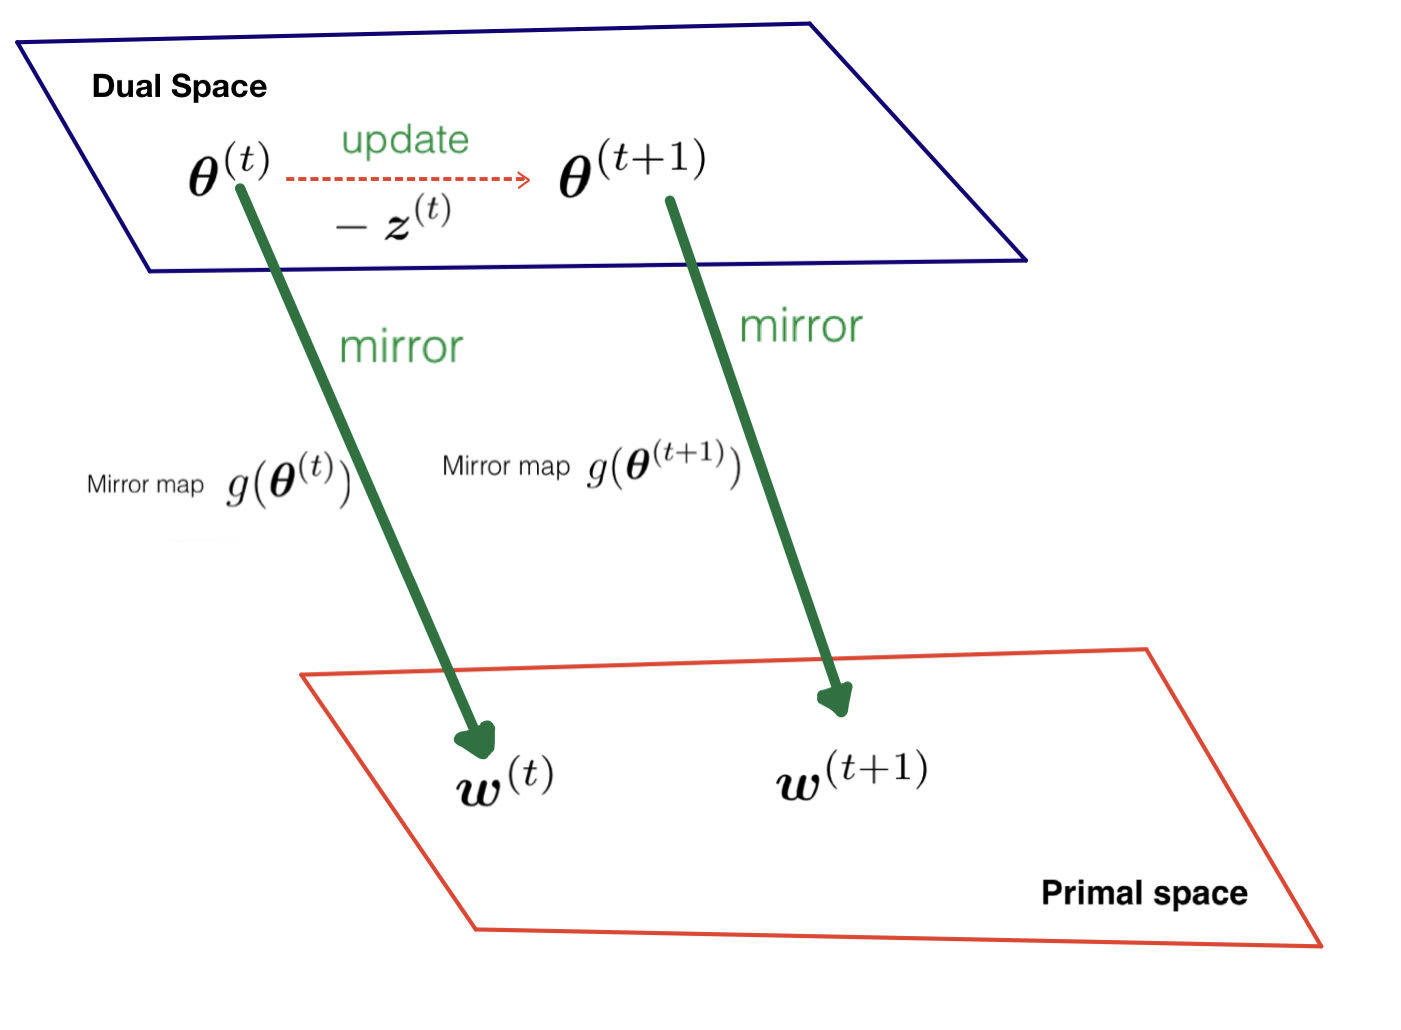
\includegraphics[width=0.6\textwidth]{geometry.jpg}
    \caption{Illustration of online mirror descent process}
    \label{fig:dual_primal}
\end{figure}

One thing to keep in mind is that different regularizations will lead to different mirror functions. We ought to choose good $g$ functions to take better advantage of the geometry of the solution space.


\subsection{Duality}
The overall topic of duality within this context relates to the phrase: "If the dual of A is B, then the dual of B is A." The subtopics of duality are convex conjugates and Bregman Divergence, two mathematical tools used to understand the OMD regret bound calculation.

\subsubsection{Convex Conjugate}
Given a primal set (i.e. parameter, function set) $\{ \psi(w), w \}$, there exists a dual set expressed in slope inputs and intercept functions $\{ b(\theta), \theta \}$. The traditional method of characterizing functions is in the primal set, where the input $w$ is mapped to a function $\psi(w)$. In the same sense of characterizing functions, one can also describe a function based on a set of line equations at each point such that each slope $\theta$ has a mapping function to output intercepts $b(\theta)$. A visualization of the dual set is shown in Figure \ref{fig:dual_set_graph} below. Given the dual equation at point $w^*$ is $\psi(w^*) = <\theta, w^*> - b$, then one can determine the intercept as a function of $\theta$ at $w^*$ such that $-b(\theta) = -<\theta, w^*(\theta)> + \psi(w^*(\theta))$.

\begin{figure}[H]
    \centering
    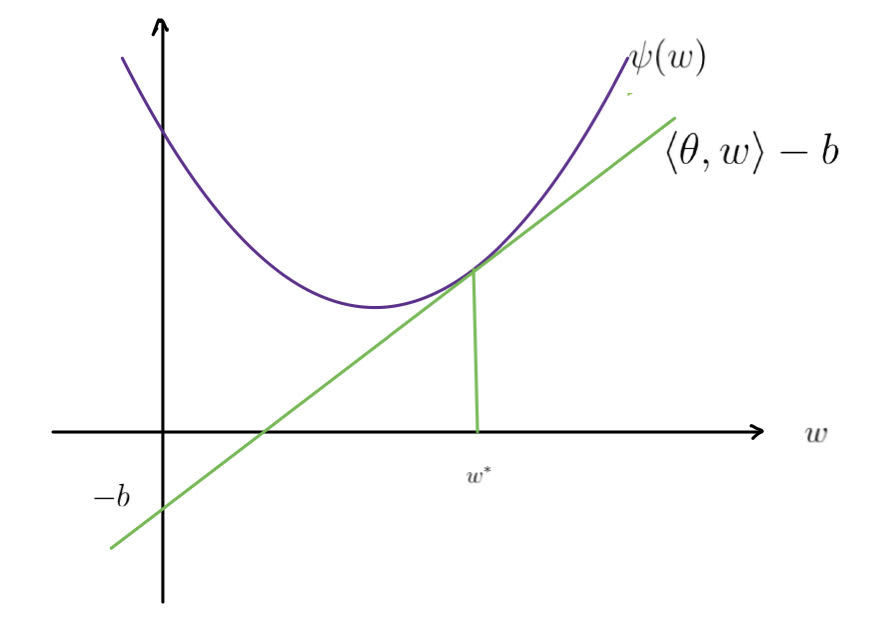
\includegraphics[width=0.6\textwidth]{f2.jpg}
    \caption{Dual set visualization}
    \label{fig:dual_set_graph}
\end{figure}

Now suppose one draws the line $<\theta, w> - \psi(w)$ through the origin, one can visualize the vertical incremental distance between points of $\psi(w)$ and the line. Computing the argument that would output the maximum distance between the sloped line and $\psi(w)$ turns out to be $w*$, or the input argument for the sloped line. A visualization is shown in Figure \ref{fig:dual_set_argmax} below. The value of that maximum distance also turns out to be $\psi^*(\theta) = \max_w (<\theta, w> - \psi(w))$. Thus, the definition of the convex conjugate function is: $\psi^*(\theta) = \max_w (<\theta, w> - \psi(w))$. 

\begin{figure}[H]
    \centering
    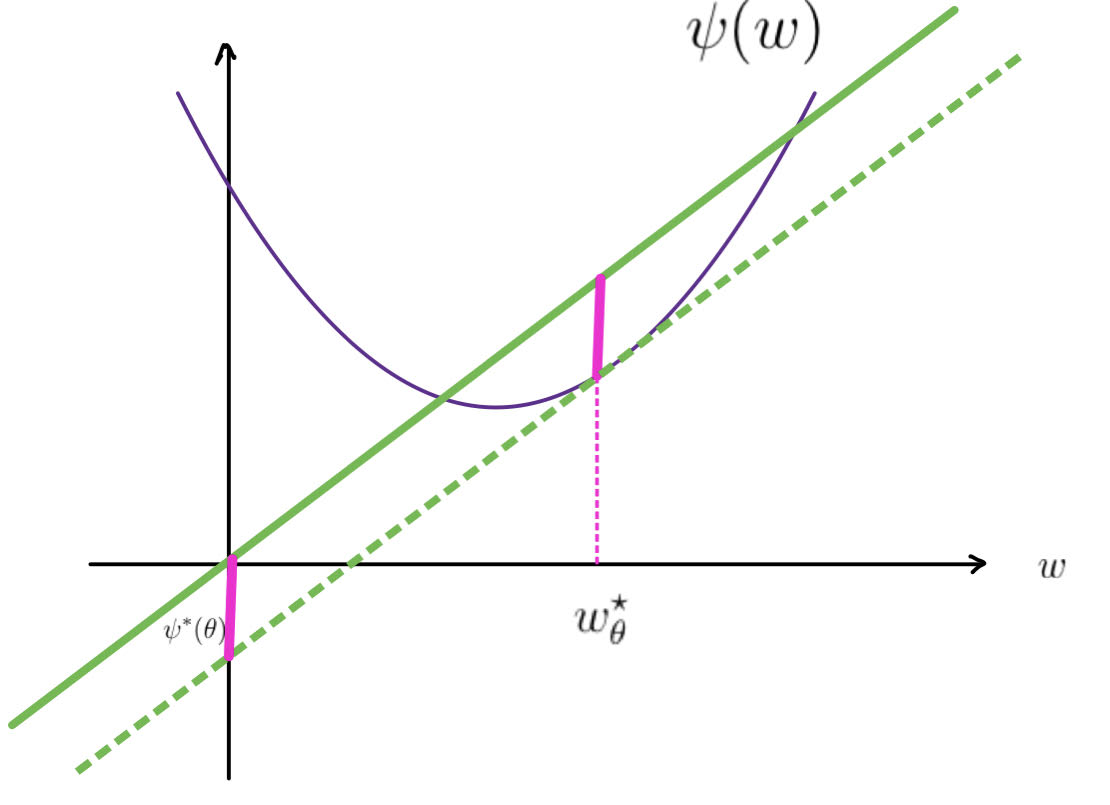
\includegraphics[width=0.6\textwidth]{f3.jpg}
    \caption{Dual set argmax illustration}
    \label{fig:dual_set_argmax}
\end{figure}

The usefulness of the convex conjugate function $\psi^*(\theta) = \max_w (<\theta, w> - \psi(w))$ comes with the various mathematical properties inherent in such a form \cite{wiki:Convex_conjugate}: 

\begin{enumerate}
    \item The derivative of the complex conjugate with respect to $\theta$ is equal to the optimal point of the function $\psi(w^*)$: $\nabla_\theta \psi^*(\theta) = \frac{\partial \psi^*(\theta)}{\partial \theta} = w^*$
    \item The derivative of the convex function with respect to $w$ is equal to the slope $\theta$: $\nabla_w \psi(w) = \frac{\partial \psi(w)}{\partial w} |_{w=w^*} = \theta$
    \item The complex conjugate computed for a specific $\theta$ input is lower bounded by the line equation with any other input $w$ (Fenchel-Young inequality): $\psi^*(\theta) \geq (<\theta, w> - \psi(w))$
\end{enumerate}

\subsubsection{Bregman Divergence}

From a high-level overview, the Bregman Divergence describes the approximation error between a linear approximation and a convex function between two input points $u$ and $w$.

Let Figure \ref{fig:bregman_divergence_graph} shown below be a visualization for the Bregman Divergence. Given two points along a convex function, the difference between the two values can be seen as the incremental rise along the line function from point $w$ to point $u$ in addition to some divergence term $D_{\psi}(w||u)$. Thus, the divergence term (i.e. Bregman Divergence) can be derived to be \cite{wiki:Bregman_divergence}:

\begin{gather*}
    \psi (w) - \psi (u) = \nabla \psi(u)^T (w-u) + D_{\psi}(w||u) \\ 
    D_{\psi}(w||u) = \psi(w) - \psi(u) - \nabla \psi(u)^T (w-u) \\ 
\end{gather*}

\begin{figure}[H]
    \centering
    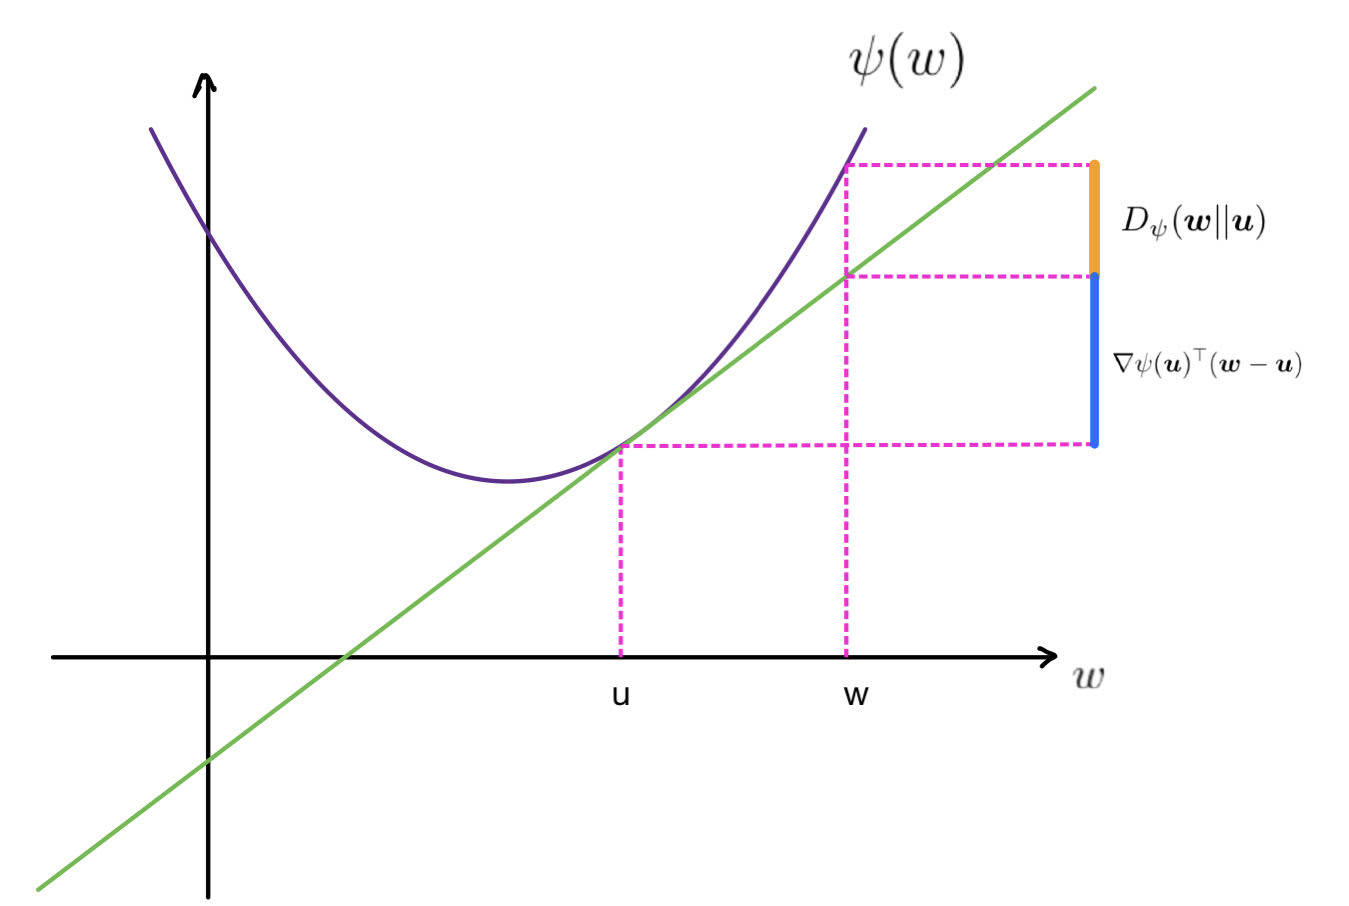
\includegraphics[width=0.8\textwidth]{f4.jpg}
    \caption{Bregman divergence graph illustration}
    \label{fig:bregman_divergence_graph}
\end{figure}

\subsection{OMD Regret Bound Analysis}

Given the aforementioned concepts of convex conjugates and the Bregman Divergence, we can now derive the regret bound for the OMD algorithm. The starting equation is the generic regret algorithm given by the following:

\begin{gather*}
    R(u) = \sum_{t=1}^T w^{(t)} \cdot z^{(t)}  - u \cdot z^{(t)}\\ 
    R(u) = \psi (u) + \sum_{t=1}^T u \cdot z^{(t)} \\ 
    R(u) = \psi (u) - u \cdot \theta^{(T+1)}
\end{gather*}

Applying the Fenchel-Young inequality gives us the following lower bound:

\begin{gather*}
    \psi (u) - u \cdot \theta^{(T+1)} \geq -\psi^* (\theta^{(T+1)})
\end{gather*}

Then, apply telescoping to the right-hand side of the inequality introduces the Bregman Divergence term. In the last line of the derivation below, the right hand side is broken up into two terms, where the second term is considered the first-order approximation of $\psi (w)$ and the third term is the Bregman Divergence.

\begin{gather*}
    -\psi^* (\theta^{(T+1)}) = -\psi^* (\theta^{(T+1)}) - \psi^* (\theta^{(1)}) + \psi^* (\theta^{(1)}) \\
    -\psi^* (\theta^{(T+1)}) = -\psi^* (\theta^{(T+1)}) - \psi^* (\theta^{(T)}) + \psi^* (\theta^{(T)}) - \dots - \psi^* (\theta^{(1)}) + \psi^* (\theta^{(1)}) \\ 
    -\psi^* (\theta^{(T+1)}) = - \psi^* (\theta^{(1)}) - \sum_{t=1}^T (\psi^* (\theta^{(t)}) - \psi^* (\theta^{(t)})) \\ 
    -\psi^* (\theta^{(T+1)}) = - \psi^* (\theta^{(1)}) - \underset{\text{$1^{st}$ order approx. of $\psi (w)$}}{\underline{\sum_{t=1}^T (\nabla \psi^* (\theta^{(t)}) \cdot (\theta^{(t+1)} - \theta^{(t)})}} + \underset{\text{Bregman Divergence}}{\underline{D_{\psi^*} (\theta^{(t+1)}||\theta^{(t)})}} \\
\end{gather*}

Substituting the definition of the convex conjugate to be $\psi^* (\theta^{(1)}) = -\psi (w^{(1)})$ and the convex conjugate derivative property $\nabla_\theta \psi^* (\theta) = w^*$, the equation becomes:

\begin{gather*}
    -\psi^* (\theta^{(T+1)}) = - \psi^* (\theta^{(1)}) - \sum_{t=1}^T (\nabla \psi^* (\theta^{(t)}) \cdot (\theta^{(t+1)} - \theta^{(t)}) + D_{\psi^*} (\theta^{(t+1)}||\theta^{(t)}) \\
    -\psi^* (\theta^{(T+1)}) = - \psi (w^{(1)}) - \sum_{t=1}^T (w^{(t)} \cdot (-z^{(1:t)} + z^{(1:t-1)}) + D_{\psi^*} (\theta^{(t+1)}||\theta^{(t)}) \\ 
    \psi^* (-z^{(1:T)}) = -\psi (w^{(1)}) - \sum_{t=1}^T <w^{(t)}, z^{(t)}> - D_{\psi^*} (-z^{(1:t)}||-z^{(1:t-1)}) \\ 
\end{gather*}

Substituting $\psi^* (-z^{(1:T)})$ back into the lower bound inequality and by rearranging terms, we are left with:

\begin{gather*}
    \psi (u) - u \cdot \theta^{(T+1)} \geq -\psi^* (\theta^{(T+1)}) \\ 
     <u, -z^{(1:T)} > - \psi (u) \leq \psi^* (-z^{(1:T)}) \\ 
     <u, -z^{(1:T)} > - \psi (u) \leq -\psi (w^{(1)}) - \sum_{t=1}^T <w^{(t)}, z^{(t)}> - D_{\psi^*} (-z^{(1:t)}||-z^{(1:t-1)}) \\ 
     -<u, z^{(1:T)} > - \psi (u) \leq -\psi (w^{(1)}) - \sum_{t=1}^T <w^{(t)}, z^{(t)}> + \sum_{t=1}^T D_{\psi^*} (-z^{(1:t)}||-z^{(1:t-1)}) \\ 
     \sum_{t=1}^T <w^{(t)}, z^{(t)}> - <u, z^{(1:T)} > \leq \psi (u) - \psi (w^{(1)}) + \sum_{t=1}^T D_{\psi^*} (-z^{(1:t)}||-z^{(1:t-1)}) 
\end{gather*}

Thus, the OMD regret bound is defined by the algorithm shown below. In the last line of the derviation on the right-hand-side, there are three terms. The first term is the regularization term, and the third term is the Bregman Divergence term under the convex conjugate of the regularization function.

\begin{gather*}
    \sum_{t=1}^T <w^{(t)}, z^{(t)}> - <u, z^{(1:T)} > \leq \psi (u) - \psi (w^{(1)}) + \sum_{t=1}^T D_{\psi^*} (-z^{(1:t)}||-z^{(1:t-1)})  \\ 
    R(u) \leq \underset{\text{regularization}}{\underline{\psi (u)}} - \psi (w^{(1)}) + \sum_{t=1}^T \underset{\text{Bregman Divergence}}{\underline{D_{\psi^*} (-z^{(1:t)}||-z^{(1:t-1)})}} \\
\end{gather*}

% \nocite{*}
\newpage
\bibliography{refs} 
\bibliographystyle{abbrv}

%\section{Appendix}
%This section provides any relevant background material that was not covered in the lectures but was found to be useful for understanding the material. 
%For example, derivations, theory underlying techniques employed, etc. 

%Additionally, this section can summarize applications or extensions of these techniques found in the literature. 

\end{document} % Done!